% !TEX root =  ../ms.tex

\section{Personalized Schedules for Measurement of SCr}
\label{sec: simulation_study}
Currently, the schedule for measurement of SCr levels and fixed and common for all patients. SCr levels are measured 20 times in the first year after transplantation and every three months thereafter. Such fixed and frequent schedules are often burdensome for the patients. Patients who remain relatively stable after transplantation may not require frequent measurement of SCr in the first year. On the other hand, patients for whom the graft decays faster after the first year, a frequent schedule of SCr may be required to check the state of the graft. In this regard, instead of a common fixed schedule for all patients, we propose using a different schedule for every patient. More specifically, we propose using personalized schedules based on JMs \citet{drizopoulosPersScreening}. This is because, JMs utilize random effects and thus they are inherently patient specific. In this direction, firstly a full specification the joint distribution of SCr levels and time of graft failure is obtained. It is then used to define a patient-specific posterior predictive distribution of time of graft failure, given the observed SCr measurements. The optimal time of the next SCr measurement is the one at which the expected information gained from an extra SCr measurement is maximum. In order to create reasonable predictions, SCr measurements for the first 3 months are taken as per the fixed schedule. This time period corresponds to the time around which we observed an increase in the SCr profile.

Since the SCr measurements are already taken for the kidney transplant patients, in order to demonstrate the efficacy of the personalized schedules we conduct a small simulation. To this end, we first assume a population of kidney transplant patients, whose SCr and hazard of graft failure follow a JM of the form described in Section \ref{sec : joint_model}, with parameters equal to the posterior mean of parameters estimated from the joint model fitted to the kidney transplant dataset. From this population we sample 625 patients, which are further split into a training (575 patients) and test (50 patients) part. For the training patients we generate a graft failure time $T^*_i$ as well as a random and non-informative censoring time $C_i$. For the test patients the graft failure time $T^*_j$ and an intervention time $T^I_j$ is generated. The intervention time is the time at which the 6 month dynamic risk of graft failure of the patient becomes larger than a certain threshold $\kappa$. The choice of $\kappa$ dictates the amount of time at hand between intervention and graft failure. In this simulation we evaluate two $\kappa$ values, namely 0.05 and 0.025. 

Our goal is to compare personalized schedule with the currently used fixed schedule of SCr measurements. To this end, we first fit a joint model of the specification described in Section \ref{sec : joint_model} to the training data set and obtain a MCMC sample from the posterior distribution of the parameters of the JM. Using the fitted JM, we then iteratively schedule SCr measurements for the test patients, until the dynamic risk of graft failure \citep{rizopoulos2011dynamic} of the patients becomes larger than the threshold $\kappa$. Let $N^I_j$ denote the number of SCr measurements conducted for the $j$-th test patient. The time difference between the observed intervention time due to the schedule ($T^S_j$) and the true intervention time, that is, the intervention offset is denoted by $O^I_j = T^S_j - T^I_j$. Lastly, the failure offset $O^*_j = T^S_j - T^*j$ is the time at hand between the observed intervention time and the time of graft failure. Using the test patients, we calculate these measures for both personalized and fixed schedules. It is to be noted that in the ideal scenario, $N^I_j$ will be one, and offset $O^I_j$ will be zero. 

\begin{figure}[!htb]
\centerline{\includegraphics[width=\columnwidth]{images/nObspt05.eps}}
\caption{Boxplot of the number of SCr measurements $N^I_j$ for the test patients, for $\kappa = 0.05$.}
\label{fig : nObspt05}
\end{figure}

\begin{figure}[!htb]
\centerline{\includegraphics[width=\columnwidth]{images/truethrestimept05.eps}}
\caption{Boxplot of the intervention offset $O^I_j$ for the test patients, for $\kappa = 0.05$. The zero offset mark is displayed with the dashed line.}
\label{fig : truethrestimept05}
\end{figure}

\begin{figure}[!htb]
\centerline{\includegraphics[width=\columnwidth]{images/truestoptimept05.eps}}
\caption{Boxplot of the failure offset $O^*_j$ for the test patients, for $\kappa = 0.05$. The zero offset mark is displayed with the dashed line.}
\label{fig : truestoptimept05}
\end{figure}


A boxplot of the observed values of the number of SCr measurements $N^I_j$, intervention offset $O^I_j$ and failure offset $O^*_j$ are presented in Figure \ref{fig : nObspt05}, Figure \ref{fig : truethrestimept05} and Figure \ref{fig : truestoptimept05}, respectively. The mean number of SCr measurements for personalized schedule is 14.46 whereas it is 27.60 for fixed schedule. In addition the standard deviation for number of SCr measurements is 9.17 for fixed schedule and 4.03 for personalized schedule. That is, personalized schedule not only schedule less $N^I_j$ on average but the variation in $N^I_j$ from patient to patient is also less. The mean absolute intervention offset for personalized schedules is 0.445 whereas for fixed schedules it is 0.448. The personalized schedule also has less standard deviation for absolute $O^I_j$, with it being 0.285 for personalized schedule and being 0.338 for fixed schedule. There is indeed a risk that either of the schedule can exceed the true graft failure time. In this regard, 12\% of the times the graft failure is not detected for the test patients when fixed schedule is used. This rate is 14\% when personalized schedule is used. Furthermore, the mean absolute failure offset is 2.71 for personalized schedule and 2.76 for fixed schedule. The standard deviation for absolute $O^*_j$ is 1.97 for personalized schedule and 2.21 for fixed schedule. 

In order to reduce the risk of overshooting the true graft failure time we propose that a smaller $\kappa$ of 0.025 is used. The boxplot for the failure offset for this scenario is displayed in Figure \ref{fig : truestoptimept025}. In this scenario only for 6\% of the patients the graft failure time is exceeded. Boxplot for number of SCr measurements $N^I_j$ and intervention offset $O^I_j$ are displayed in Figure \ref{fig : nObspt025} and Figure \ref{fig : truethrestimept025}, respectively. However in this scenario, although the personalized schedule conducts less SCr measurements, it also exceeds the true intervention time more often than the fixed schedule.

\begin{figure}[!htb]
\centerline{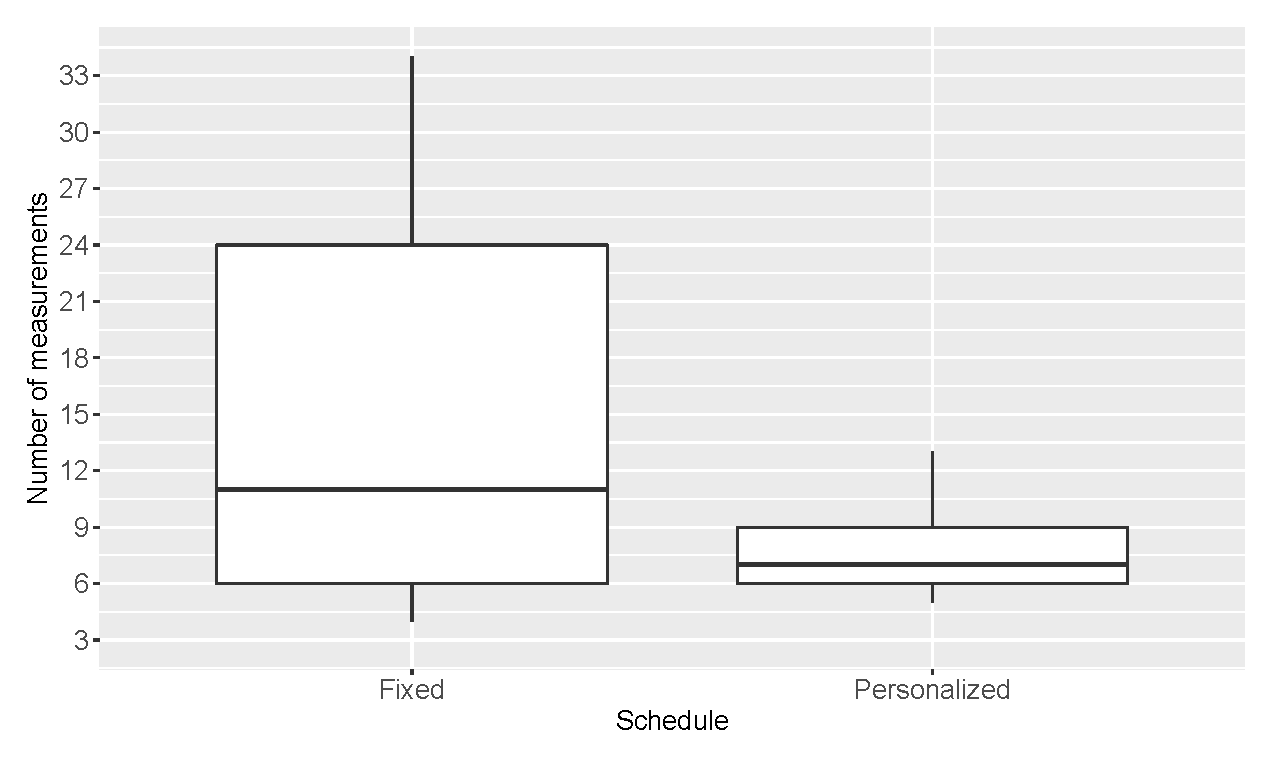
\includegraphics[width=\columnwidth]{images/nObspt025.eps}}
\caption{Boxplot of the number of SCr measurements $N^I_j$ for the test patients, for $\kappa = 0.025$.}
\label{fig : nObspt025}
\end{figure}

\begin{figure}[!htb]
\centerline{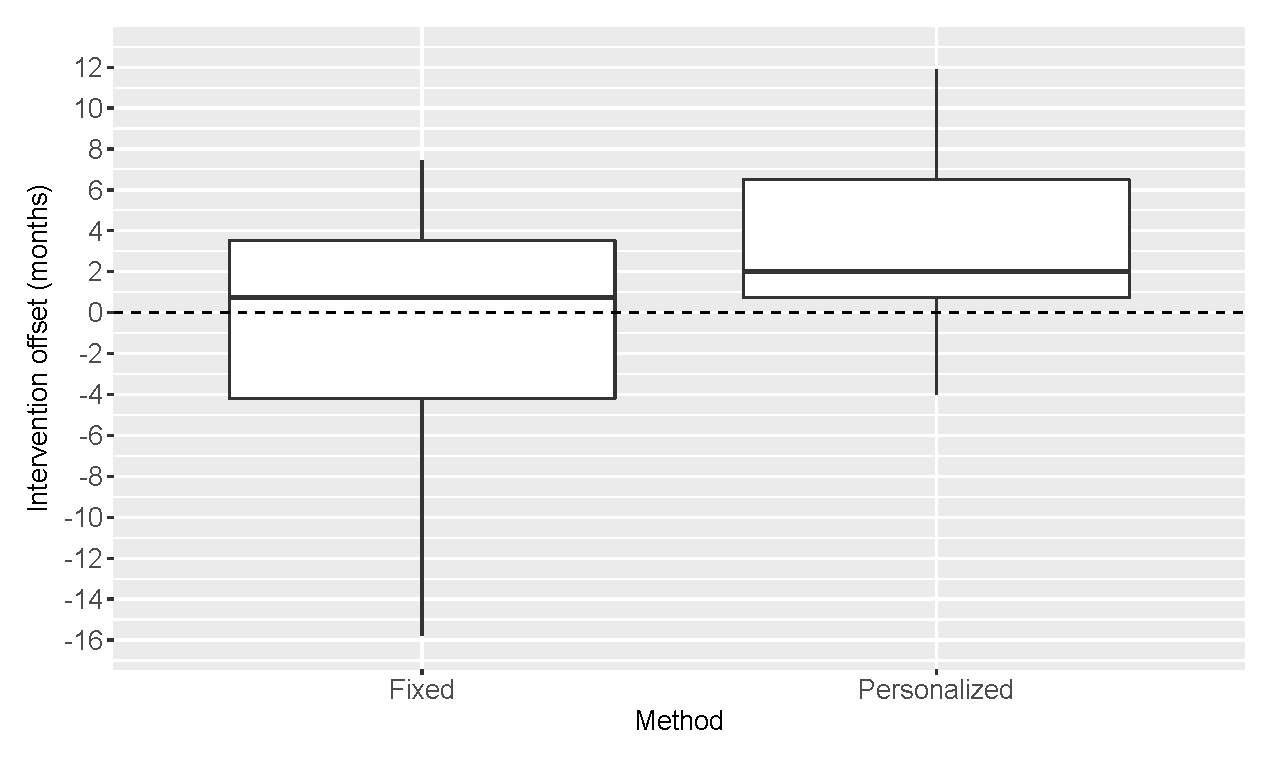
\includegraphics[width=\columnwidth]{images/truethrestimept025.eps}}
\caption{Boxplot of the intervention offset $O^I_j$ for the test patients, for $\kappa = 0.025$. The zero offset mark is displayed with the dashed line.}
\label{fig : truethrestimept025}
\end{figure}

\begin{figure}[!htb]
\centerline{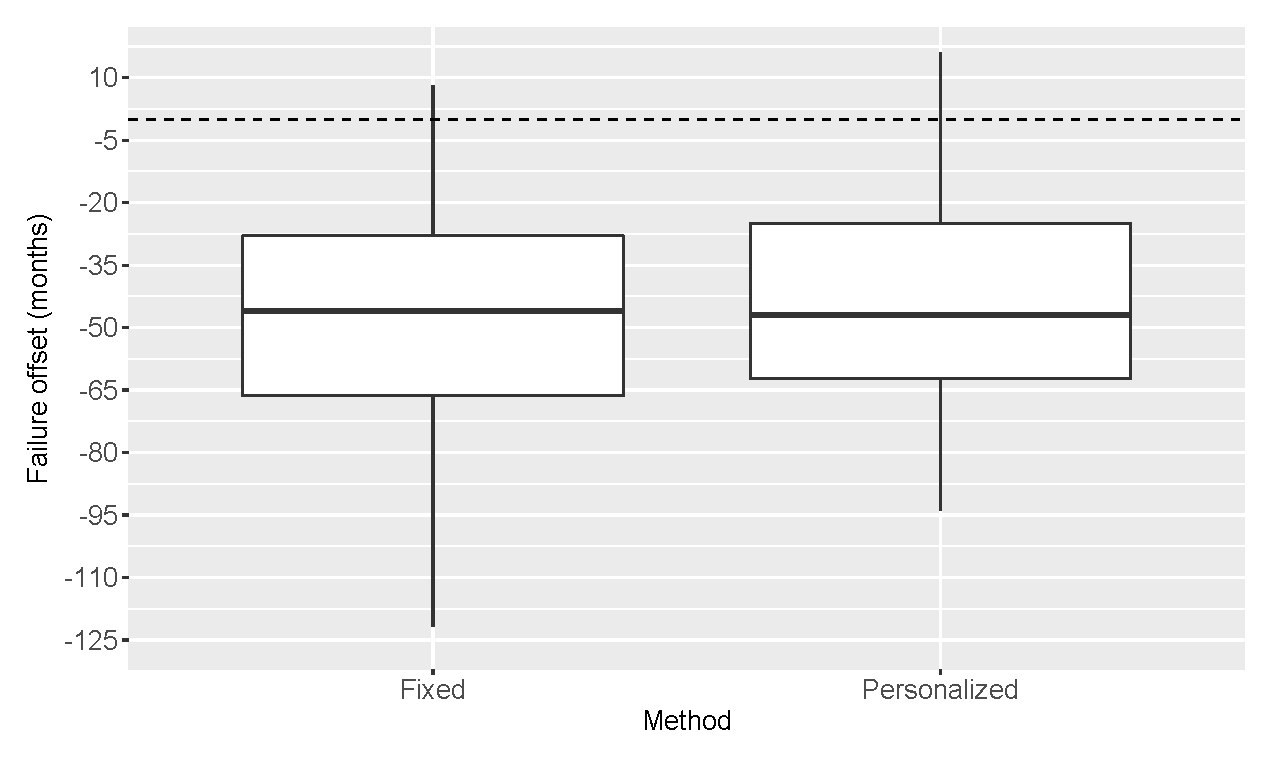
\includegraphics[width=\columnwidth]{images/truestoptimept025.eps}}
\caption{Boxplot of the failure offset $O^*_j$ for the test patients, for $\kappa = 0.025$. The zero offset mark is displayed with the dashed line.}
\label{fig : truestoptimept025}
\end{figure}